\chapter{Interrupt}

阅读代码需要一个开始的地方,因为PicoBlaze定位是可编程状态机,
那么就从外部中断开始阅读,中断包含同步、使能、上下文切换。

先介绍同步模块“interrupt\_capture”。


\section{int\_capture\_flop}
我们先从外部中断引脚开始看,看看经过哪些器件。以下是picoblaze的顶层接口:

\begin{vcode}
module kcpsm3(
        address,
        instruction,
        port_id,
        write_strobe,
        out_port,
        read_strobe,
        in_port,
        interrupt,
        interrupt_ack,
        reset,
        clk) ;
 
output  [9:0]   address ;
input   [17:0]  instruction ;
output  [7:0]   port_id ;
output          write_strobe, read_strobe, interrupt_ack ;
output  [7:0]   out_port ;
input   [7:0]   in_port ;
input           interrupt, reset, clk ;
\end{vcode}


\newpage
可以从字义上理解interrupt为外部中断的入口,而interrupt\_ack为中断确认信号,interrupt首先连入int\_capture\_flop逻辑:

\begin{vcode}
// Interrupt capture
FDR int_capture_flop (
    .D(interrupt),
    .Q(clean_int),
    .R(internal_reset),
    .C(clk));
\end{vcode}

这个FDR是“同步复位D触发器”原语。FDR是比较好理解的,D是输入,Q是输出,R是复位,C是时钟。\\
在\verb|C:\Xilinx\12.4\ISE_DS\ISE\verilog\xeclib\unisims|下是官方给出的仿真代码。
在后面还会涉及到LUT(查找表),所以在这里先介绍一下。

\textbf{FDR}
\begin{vcode}
module FDR (Q, C, D, R);
    parameter INIT = 1'b0;
    output Q;
    reg    Q;
    input  C, D, R;
    always @(posedge C)
        if (R)
        Q <= 0;
        else
        Q <= D;
endmodule
\end{vcode}

\textbf{LUT4}
\begin{vcode}
module LUT4 (O, I0, I1, I2, I3);
    parameter INIT = 16'h0000;
    input I0, I1, I2, I3;
    output O;
    wire out0, out1, out2, out3, out;
    assign O = INIT[{I3,I2,I1,I0}];
endmodule
\end{vcode}

可以看出就是一个16bit的ROM结构,O是输出,I3、I2、I1、I0是地址线。
因为原语不太直观,所以在这里把\verb|int_capture_flop|改写为rtl描述。

\begin{vcode}
always@(posedge clk)
begin
    if (internal_reset)
        clean_int <= 1'b0;
    else
        clean_int <= interrupt;
end
\end{vcode}

在Synplify的Technology View可以看到如下的图\\
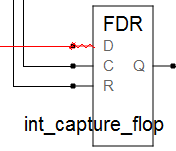
\includegraphics{images/int_capture_flop.png}

这个逻辑同步外部的中断信号。interrupt是外部中断信号,\verb|clean_int|是同步后的中断信号。 \verb|internal_reset|是PicoBlaze内部复位信号,当处理器复位的时候,\verb|internal_reset|会持续一段时间。

用原语来写有个好处就是综合的结果基本上就是你想要的电路,
但是代价就是不容易维护,也不利于别人阅读。

\clearpage
\section{Karnaugh Graphic}
用原语来写就涉及到自己优化逻辑的问题,就需要理解卡诺图了,
而阅读用原语写的组合逻辑代码就更痛苦了,
因为LUT的值是一个16位的数字,很不直观这就要自己写个脚本
把16位的值转为一个平面的图。

\textbf{karnaugh.py}
\begin{pythoncode}
#!/bin/python
import sys

def itob(a, bitnum=16):
    bits = []
    for i in range(0, bitnum):
        if (a & (1 << (bitnum - 1 - i))) != 0:
            bits.append('1')
        else:
            bits.append('0')
    return bits

def printv(bits):
    #dec format index
    sys.stdout.write('bitno: ')
    for i in range(15, -1, -1):
        sys.stdout.write('%4d' % i)
        if (i % 4) == 0:
            sys.stdout.write(' | ')
        else:
            sys.stdout.write(' ')
    sys.stdout.write('\n')

    #binary format index
    sys.stdout.write('bitno: ')
    for i in range(15, -1, -1):
        sys.stdout.write(''.join(itob(i, bitnum=4)))
        if (i % 4) == 0:
            sys.stdout.write(' | ')
        else:
            sys.stdout.write(' ')
    sys.stdout.write('\n')

    #value
    sys.stdout.write('value: ')
    bitno = 15
    for bit in bits:
        sys.stdout.write('%4s' % bit)
        if (bitno % 4) == 0:
            sys.stdout.write(' | ')
        else:
            sys.stdout.write(' ')
        bitno -= 1
    sys.stdout.write('\n')
    sys.stdout.write('\n')

    #karnaugh map
    print('kano-graphic:')
    sys.stdout.write('||= bit(3210) =|' + \
            '|=  xx11 =||=  xx10 =||=  xx00 =||=  xx01 =||\n')
    
    sys.stdout.write('||         11xx||%7s  ||%7s  ||%7s  ||%7s  ||\n' % (
        bits[0*4 + 0], bits[0*4 + 1], bits[0*4 + 3], bits[0*4 + 2]))
    
    sys.stdout.write('||         10xx||%7s  ||%7s  ||%7s  ||%7s  ||\n' % (
        bits[1*4 + 0], bits[1*4 + 1], bits[1*4 + 3], bits[1*4 + 2]))
    
    sys.stdout.write('||         00xx||%7s  ||%7s  ||%7s  ||%7s  ||\n' % (
        bits[3*4 + 0], bits[3*4 + 1], bits[3*4 + 3], bits[3*4 + 2]))
    
    sys.stdout.write('||         01xx||%7s  ||%7s  ||%7s  ||%7s  ||\n' % (
        bits[2*4 + 0], bits[2*4 + 1], bits[2*4 + 3], bits[2*4 + 2]))
    sys.stdout.write('\n')

def printlut4(a):
    bits = itob(a)
    print('original: 0x%04X' % a)
    print
    printv(bits)

if __name__ == '__main__':
    if len(sys.argv) == 1:
        print 'need hex digit!'
    else:
        printlut4(int(sys.argv[1], 16))

\end{pythoncode}



对于0x1010,转换的结果如下:
\begin{textcode}
kano-graphic:
||= bit(3210) =||=  xx11 =||=  xx10 =||=  xx00 =||=  xx01 =||
||         11xx||      0  ||      0  ||      1  ||      0  ||
||         10xx||      0  ||      0  ||      0  ||      0  ||
||         00xx||      0  ||      0  ||      0  ||      0  ||
||         01xx||      0  ||      0  ||      1  ||      0  ||
\end{textcode}


